%\documentclass[oneside, DIV=11, BCOR=10mm]{scrbook}
\documentclass[oneside]{scrbook}
\usepackage[english]{babel}
\usepackage[T1]{fontenc}
\usepackage{amsmath}
\usepackage{booktabs}
\usepackage{mathtools}
\usepackage{graphicx}
\usepackage{xspace}
\usepackage{cite}
\usepackage[xindy,toc]{glossaries}
\usepackage{todonotes}
\usepackage{units}
\usepackage{xstring}
\usepackage[round,colon]{natbib}
\usepackage[activate={true,nocompatibility}]{microtype}
% code listings
\usepackage{listings}
\usepackage{multicol}
\usepackage{url}
\usepackage{bytefield}
\usepackage{algpseudocode}
\lstset{
    basicstyle=\footnotesize\ttfamily,
    numbers=left,
    numberstyle=\tiny,
    %stepnumber=5,
    numbersep=5pt,
    tabsize=2,
    breaklines=true,
    xleftmargin=17pt,
    framexleftmargin=17pt,
    framexrightmargin=5pt,
    framexbottommargin=4pt
}
\lstloadlanguages{c}
% clickable links
\usepackage[
  pdftex,
  pdfauthor={Simon Friedmann},
  pdftitle={Plasticity Processor User Guide}
]{hyperref}
\hypersetup{
  hidelinks=true,
  colorlinks=false,
  urlcolor=black,
  linkcolor=black,
  citecolor=black
}
% font selection
\usepackage{mathpazo}
\usepackage[scaled]{berasans}
\usepackage{courier}

\title{Universal Neuromorphic Instruction set}
\author{Simon Friedmann}

%
% Glossaries
%
\makeglossaries
\loadglsentries{src/glossaries.tex}

%
% custom macros
%

% template to typeset identifiers from code containing _ and :: characters
\newcommand{\code}[1]{\texttt{%
    \noexpandarg %
    \StrSubstitute{#1}{_}{\textunderscore}[\x]%
    \expandafter\StrSubstitute\expandafter{\x}{::}{$\dblcolon$}[\x]%
    \x}\xspace}

% template for file references
\newcommand{\file}[1]{\path{#1}\xspace}



\begin{document}

	\maketitle
    \tableofcontents

    \chapter{Introduction}

\section{Scope of this document}

This document provides high-level overview of the \gls{uni}.
It specifies the instruction format and execution model.
Detailed description of the implementation in software and hardware is beyond the scope.


\section{Further reading}

There is Doxygen generated documentation for source code in \file{doc/doxygen}.


\section{Basic ideas}

\Gls{uni} addresses a basic problem for real-time neuromorphic hardware systems:
Stimulus such as spikes and often also configuration data has to be delivered with predictable and bounded timing.
A standard method to do this, is to store stimulation data with timing information in \gls{sdram} on an \gls{fpga} and then play it back in one go.
Result data, i.e.\ spikes generated by the hardware and responses to read requests must also be recorded with annotated timing information.
This approach allows for batch execution of experiments: load stimulus program, execute experiment, read back result data.
Further operation modes for neuromorphic hardware are continuous streaming of input stimulus and result data and recurrent communication between components of the neuromorphic hardware system.

\Gls{uni} is designed to provide all three modes of operation simultaneously in one hardware implementation.
At its core it is an instruction set definition for byte-code that defines stimulus data with timing information together with an execution model for this byte-code.
The same coding is used to encode result data.
An important characteristic of this byte-code is its independence of a particular neuromorphic hardware system (the back-end).
Instead it provides instructions for timing control, reading and writing configuration data, and for event delivery.
The back-end defines the semantics of these operations and the actual \gls{fpga} implementation of \gls{uni} performs the translation to the concrete back-end interface.

Streaming operation is enabled through double buffering: while one batch of stimulus data is being executed, the host computer transfers the next batch.
The implementation provides gap-free back-to-back execution between buffer switches.
Recurrent connections provide additional events that have to be delivered with low-latency to their destination.
This is realized by mixing units that combine event streams from within the system with batch streams coming from memory.


\section{Terms and definitions}

Here are a couple of definitions for this document:

\begin{description}
    \item[Back-end]
        A particular neuromorphic hardware system that is to be controlled and stimulated.

    \item[Instruction]
        An atomic operation for execution in the back-end or timing control.

    \item[Byte-code]
        A sequence of instructions in binary form.
        Instructions are coded in one or more byte.

    \item[Program]
        The sequence of configuration accesses and spike-events with their timing information is called a program.
        The implementation executes the program, i.e.\ plays it back to the back-end using the given timing information.
        The program is a sequence of instructions and represented as byte-code.

    \item[Implementation]
        A concrete realization of the \gls{uni} specification for a particular back-end.

    \item[Execution model]
        Defines how the program in its byte-code representation is executed in a \gls{uni} implementation.

    \item[Data frame]
        Back-end specific atomic unit of data for transfer to the neuromorphic system.
\end{description}



    \chapter{Instruction set}

This chapter specifies the execution model for programs and the format of byte-code.


\section{Execution model}
\begin{figure}
    \centering
    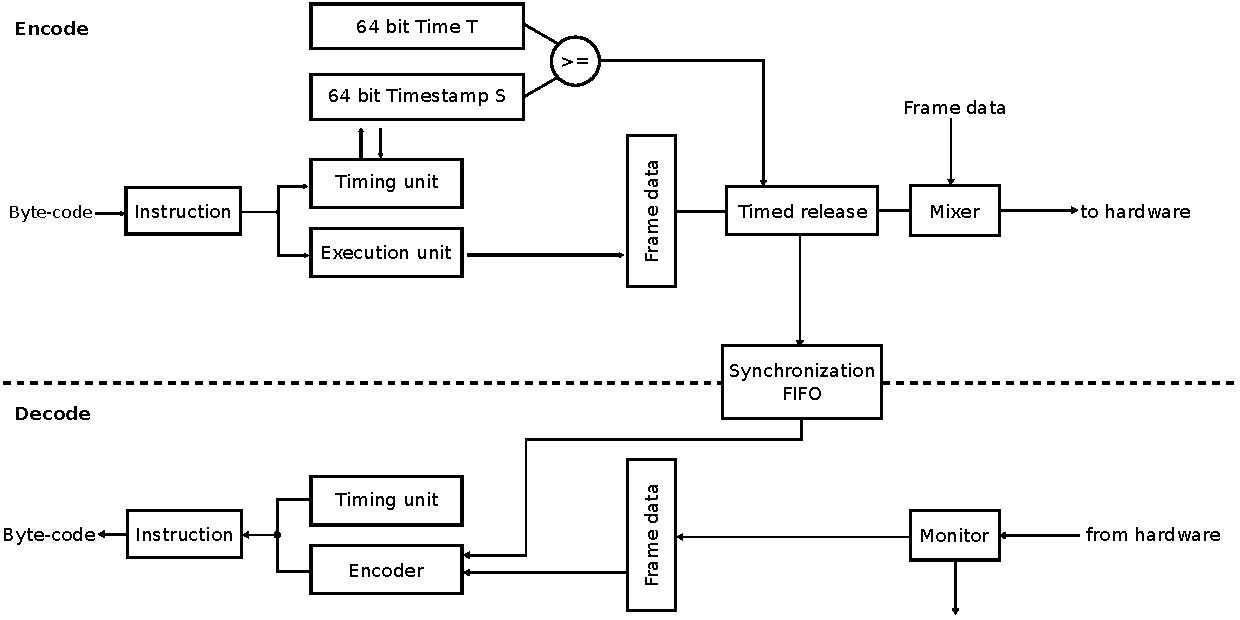
\includegraphics[width=\textwidth]{figures/dataflow.pdf}
    \caption{%
        Dataflow in the execution model.
    }
    \label{fig:dataflow}
\end{figure}

Figure~\ref{fig:dataflow} shows the flow of data within the \gls{uni} execution model.
There is an encode and a decode path.
The encode path takes byte-code as input, decodes the contained instructions and issues them either to the timing or the execution unit.

The timing unit handles all aspects of temporal control: setting of the global system timer and specifying the execution time for the next operation send to the execution unit.
The global system timer $T$ is a \unit[64]{bit} counter that increments in each clock cycle.
The timing unit can initialize this $T$.
The timestamp register $S$, specifies the execution time for the next operation in the execution unit.
Operations are only executed when the timer condition $S \ge T$ is true.

The execution unit converts generic \gls{uni} instructions to specific data frames for the back-end.
The timed-release block forwards frame data to the mixer and thereby the hardware when the timer condition is met.
It also pushes an entry into the synchronization \gls{fifo} if necessary.
For example a read request pushes its address into the \gls{fifo}, so that the decode path can provide this address together with the result data, when the response arrives from hardware.

The decode path converts data frames from hardware into valid byte-code including timing information using the global system timer.
Read instructions in the program are converted to write instructions in the result stream and vice versa.
The data part of the write then corresponds to the returned data from the read request.
The main reason for this is to avoid treating result data differently from program data in software and hardware.
It might also be interesting to reapply result data as program.

\textbf{Note:} So far, mixer and monitor have not been implemented.
The mixer merges data frame streams from timed release and an external port using a suitable arbitration scheme.
The monitor copies data frames to an external port.
This approach allows additional back-end specific logic to realize recurrent connections by connecting to these external ports.
They are positioned after and before buffering \glspl{fifo} respectively to minimize latency.



\section{Byte-code definition}

Instructions are one or more bytes, i.e.\ \unit[8]{bit}, long.
The first byte specifies the operation, while the remaining bytes are data.


\subsection{Implementation defined functions}

To map the generic instructions to the specific back-end two functions are to be defined by the implementation:
\begin{description}
    \item[$\text{\sc{io}}(a)$]
        Represents the contents of the \gls{io} space location at address $a$.
        This could for example be the contents of a configuration register that is addressed with the given address.

    \item[$\text{\sc{fire}}(i, a)$]
        Trigger a spike event for target $i$.
        Each event has also an address $a$.
\end{description}



\subsection{Timing control instructions}

\subsubsection{Set global system timer}
\begin{bytefield}[bitwidth=0.6em]{72}
    \bitheader{0,7,8,71} \\
    \bitbox{8}{$0000 0000$} & \bitbox{64}{$t$} \\
\end{bytefield} \\
\textbf{\code{SET_TIME}}
{\footnotesize
\begin{algorithmic}[1]
    \State $T \gets t$
\end{algorithmic} }
Set the global system timer $T$ to the specified value $t$.
The most significant bit of $t$ is at position 8.


\subsubsection{Wait until}
\begin{bytefield}[bitwidth=0.6em]{72}
    \bitheader{0,7,8,71} \\
    \bitbox{8}{$0000 0000$} & \bitbox{64}{$t$} \\
\end{bytefield} \\
\textbf{\code{WAIT_UNTIL}}
{\footnotesize
\begin{algorithmic}[1]
    \State $S \gets t$
\end{algorithmic} }
Set the timestamp $S$ to the specified value $t$.
The most significant bit of $t$ is at position 8.
This delays the next instruction for the execution unit to the time $t$.


\subsubsection{Wait for}
\begin{bytefield}[bitwidth=0.6em]{8}
    \bitheader{0,1,7} \\
    \bitbox{1}{$1$} & \bitbox{7}{$t$} \\
\end{bytefield} \\
\textbf{\code{WAIT_FOR_7}}
\vspace{2em}

\begin{bytefield}[bitwidth=0.6em]{24}
    \bitheader{0,7,8,23} \\
    \bitbox{8}{$0000 0100$} & \bitbox{16}{$t$} \\
\end{bytefield} \\
\textbf{\code{WAIT_FOR_16}}
\vspace{2em}

\begin{bytefield}[bitwidth=0.6em]{40}
    \bitheader{0,7,8,39} \\
    \bitbox{8}{$0000 0101$} & \bitbox{32}{$t$} \\
\end{bytefield} \\
\textbf{\code{WAIT_FOR_32}}
\vspace{2em}

{\footnotesize
\begin{algorithmic}[1]
    \State $S \gets S + t$
\end{algorithmic} }
Increment timestamp $S$ by the specified amount $t$.
The most significant bit of $t$ is at position 1.
This delays the next instruction for the execution unit to the new value of the timestamp register.


\subsection{Configuration instructions}


\subsubsection{Write}
\begin{bytefield}[bitwidth=0.6em]{72}
    \bitheader{0,7,8,39,40,71} \\
    \bitbox{8}{$0000 1010$} & \bitbox{32}{$a$} & \bitbox{32}{$d$} \\
\end{bytefield} \\
\textbf{\code{WRITE}}
{\footnotesize
\begin{algorithmic}[1]
    \State $\Call{io}{a} \gets d$
\end{algorithmic} }
Write to back-end address space.
This creates a matching \code{READ} instruction in the result stream with address $a$.


\subsubsection{Read}
\begin{bytefield}[bitwidth=0.6em]{40}
    \bitheader{0,7,8,39} \\
    \bitbox{8}{$0000 1011$} & \bitbox{32}{$a$} \\
\end{bytefield} \\
\textbf{\code{READ}}
{\footnotesize
\begin{algorithmic}[1]
    \State $y \gets \Call{io}{a}$
\end{algorithmic} }
Read from back-end address space.
This creates a matching \code{WRITE} instruction in the result stream with address $a$ and data $y$.



\subsection{Event instructions}


\subsubsection{Fire}
\begin{bytefield}[bitwidth=0.5em]{80}
    \bitheader{0,7,8,71,79} \\
    \bitbox{8}{$0000 1111$} & \bitbox{64}{$s$} & \bitbox{8}{a} \\
\end{bytefield} \\
\textbf{\code{FIRE}}
{\footnotesize
\begin{algorithmic}[1]
    \For{ $0 \le i < 64$ }
        \If{s[i] = 1}
            \State \Call{fire}{i,a}
        \EndIf
    \EndFor
\end{algorithmic} }
Send events to all targets, for which the corresponding bit in $s$ is set.
All events have the address $a$.


\subsubsection{Fire one}
\begin{bytefield}[bitwidth=0.6em]{16}
    \bitheader{0,1,2,7,8,15} \\
    \bitbox{2}{$01$} & \bitbox{6}{i} & \bitbox{8}{a} \\
\end{bytefield} \\
\textbf{\code{FIRE_ONE}}
{\footnotesize
\begin{algorithmic}[1]
    \State \Call{fire}{i,a}
\end{algorithmic} }
Send event with address $a$ to the target specified by index $i$.



\subsection{System instructions}

\subsubsection{Halt}
\begin{bytefield}[bitwidth=0.6em]{8}
    \bitheader{0,7} \\
    \bitbox{8}{$0000 1110$} \\
\end{bytefield} \\
\textbf{\code{HALT}}

Terminate program execution.


\subsubsection{Raw mode}
\begin{bytefield}[bitwidth=0.5em]{80}
    \bitheader{0,7} \\
    \bitbox{8}{$0000 0010$} & \bitbox{72}{$d$} \\
\end{bytefield} \\
\textbf{\code{RAW}}

Directly send the data frame $d$ to the hardware system.
The size of $d$ is implementation defined.


\subsubsection{Start recording}
\begin{bytefield}[bitwidth=0.6em]{8}
    \bitheader{0,7} \\
    \bitbox{8}{$0000 1100$} \\
\end{bytefield} \\
\textbf{\code{REC_START}}

Start recording in raw mode.
In raw mode, all incoming data frames are coded using \code{RAW} instructions.


\subsubsection{Stop recording}
\begin{bytefield}[bitwidth=0.6em]{8}
    \bitheader{0,7} \\
    \bitbox{8}{$0000 1101$} \\
\end{bytefield} \\
\textbf{\code{REC_STOP}}

Stop recording in raw mode.
In raw mode, all incoming data frames are coded using \code{RAW} instructions.



    %\bibliographystyle{plainnat}
    %\bibliography{src/bibliography}

\end{document}
